\subsection{Вхід алгоритму}

Для опису алгоритму створення панорамних слайдів потрібно визначити 
вхідні дані та параметри, які буде надавать користувач інформаційної
технології.

Дошка - це плоска поверхня, яку знімає камера. Це може бути крейдяна 
дошка, маркерна дошка, стіна тощо.

Записи - це ті місця дошки, де відбулася зміна кольору, яка тривала 
відносно довгий час. Важливо зауважити, що ці записи мають бути 
саме у площині дошки, при чому людина яка проходить біля неї не вважається
зміною кольору, оскільки цей рух був не тривалим.

В область огляду камери має потрапляти дошка або її частина. Наведений 
алгоритм не розрахований на відео, що містить декілька дошок, які знаходяться
не в одній плоскій площині. Камера, що знімає це відео, може рухатись, проте 
чим більше вона нерухома, тим краще: алгоритм не буде працювати, якщо камера 
рухається постійно. Дошка на відео може перекриватися сторонніми об’єктами, 
проте бажано, щоб ці об’єкти були рухливими, щоб алгоритм виявлення рухомих 
об’єктів їх помічав.

Кадром під номером $i$ шириною $w$ і висотою $h$ називаємо відображення, де 
$P$$\to$$C$, де $P$ - множина координат пікселів, $С$ - скінченна множина можливих рівнів
яскравостей (інтенсивностей) пікселів.
\begin{equation}
    P = [1, \ldots ,w]\times[1, \ldots, h], C \subset R
\end{equation},

Відео \(F\) довжиною \(T\)
є послідовністю \(\left( F^{i}:i = \overline{1,T} \right)\) кадрів
\(F^{i}:P \rightarrow C\). Той факт, що піксель з координатою
\(p \in P\) на кадрі \(F^{i}\) має інтенсивність \(c \in C\),
позначатимемо \(F_{p}^{i} = c\).


\subsection{Прибирання викладача з відео}

Під час лекцій часто виникають такі ситуації, коли викладач затуляє
собою частину дошки з написами -- наприклад, для запису нового матеріалу
або щоб видалити старі написи з дошки. Іноді студенти просять викладача
відійти від дошки, щоб переписати з неї те, що з'явилося на ній лише
хвилину тому, проте наша програма дозволяє побачити частину дошки, яку
затулив викладач, якщо перед цим перекритий сегмент було добре видно
протягом вказаного користувачем часу.

Якщо вирішити проблему прибирання викладача з відео, то студент завжди 
буде бачити, що відбувається на дошці.

Для вирішення цієї задачі ми застосовуємо декілька методів.
Що значить:
\begin{enumerate}
    \item Можна будувати маску рухомих об'єктів,
          щоб потім їх видаляти. Рухомими об'єктами можуть бути викладач, 
          студенти, а також записи, що тільки-но з'явились.
          Для цього ми вирішуємо задачу мінімального зрізу або максимального потоку
          шляхом використання алгоритму Бойкова-Колмогорова.
    \item Застосувати нейронну мережу YOLO для локалізування людини
          і подалюшої сегментації дошки та викладача.
\end{enumerate}

Розпишемо теоретичні частини кожного зі способів.

\subsection{Задача знаходження Min-Cut/Max-Flow}

Ведемо позначення:
$T$ - множина вузлів графу (рис. \ref{fig:graph_example}), 
$\tau$ - множина направлених дуг,
$s$ - джерело (початок),
$e$ - стік (кінець),
$N_t = \{t^{'}: tt^{'} \in \tau \}$,
$P_t = \{t^{'}: t^{'}t \in \tau \}$,
$f$ - потік,
$c$ - пропускна здатність,

\begin{figure}[h]
    \centering
    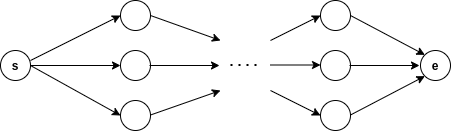
\includegraphics[width=0.6\textwidth]{images/graph_example}
    \caption{Приклад графу}
    \label{fig:graph_example}
\end{figure}

Задача максимального потоку

\begin{equation}
    \sum_{t \in N_s} f_{st} \rightarrow \max_{f: \tau \rightarrow R }
\end{equation}

З обмеженнями: 
\begin{equation} 
    \begin{gathered}
        \begin{cases}
            f_{tt^{'}} \leq  c_{tt^{'}}, &  \forall tt^{'}  \in \tau , \\

            \sum_{p \in P_t} f_{pt} - \sum_{t^{'} \in N_t} f_{tt^{'}} = 0, & 
            \forall t \in T \setminus \{s,e\}, \\

            \sum f_{tt^{'}} \geq 0, & \forall tt^{'}  \in \tau
        \end{cases}
\end{gathered}
\end{equation}

Що значить:
\begin{enumerate}
    \item Потік має не перевищувати пропускну здатність для всіх ребер;
    \item Сума потоків, що входять у вузол не повинна змінитись на виході;
    \item Потік завжди додатній.
\end{enumerate}

Оригінальний алгоритм:

\begin{algorithm}[H]
    \caption{Алгоритм Min-Cut/Max-Flow}
    \begin{algorithmic}
    \State \textbf{Вхід:} Граф, з об'єктами $t \in T$, ребрами $tt^{'}$
    \State \textbf{Вихід:} $F_{maxflow}$ - значення максимального потоку;
    \State \textbf{Ініціалізація}: $F_{maxflow} = 0, f_{tt^{'}}^{0} = 0 \quad  \forall tt^{'}  \in \tau$.
    \State \textbf{Поки існує шлях з $s$ в $e$ повторюємо кроки 1,2}:    
    \State \textbf{Крок 1}: Знаходимо шлях від $s$ до $e$.
    (алгоритм Едмонса-Карпа або Форда Фалкерсона).
    \State Відвідуємо $t^{'}$ із $t$ якщо:
            \State \qquad 1. $f_{tt^{'}} \neq   c_{tt^{'}}$
            \State \qquad 2. $ \nexists p_{t^{'}}^{i} \Rightarrow  p_{t^{'}}^{i} = t $ (запам'ятали вершину)
            \State \qquad 3. $ t^{'} \neq s $
    \State \textbf{Крок 2}: Проходимо по заданому шляху: 
            \State \qquad 1. Знаходимо $ \vartriangle f^{i} = \min_{tt^{'} \in \{шлях із s в e \}} $
            \State \qquad 2. Змінюємо потік: $ f_{tt^{'}}^{i+1} = f_{tt^{'}}^{i} + \vartriangle f^{i} $
            \State \qquad 3. Оновлюємо $F_{maxflow}$: $ F_{maxflow}^{i+1}  = F_{maxflow}^{i} + \vartriangle f^{i} $ 
    \end{algorithmic}

Знайшовши максимальний потік можемо знайти мінімальний зріз:
Для $\forall t \in T$ знайти $\theta_{t} \in \{0,1\}$
    \begin{algorithmic}
    \State \textbf{Крок 3}: Запускаємо пошук в ширину або глибину вже з оновленим графом.   
    \State \qquad Якщо $c_{tt^{'}} \geqslant f_{tt^{'}}$ та $c_{tt^{'}} \geqslant 0$
    $\Rightarrow \theta_{t^{'}} = 1 $, інакше $\theta_{t^{'}} = 0 $
    \end{algorithmic}
\end{algorithm}

У 2004 році Юрій Бойков та Володимир Колмогоров запропонували модификацію вищеописаного
методу.
Запропонована ідея методу полягає в огментації шляхів. Будується два дерева $S$ та $T$
коренями яких є $s$ та $t$ відповідно. Вершини загально діляться на ті що в $S$, $T$, та 
\textit{вільні}. Кожне дерево має \textit{активні} та \textit{внутрішні} вершини.
Алгоритм складається зі стадій \textit{росту}, \textit{огментації}, \textit{всиновлення}.\\
Коротко розглянемо кожну з них:

\begin{enumerate}
    \item \textbf{Стадія Росту}. \\
        Відбувається одночасний ріст дерев з вершин $s$ та $e$ знаходячі активні
        вершини і додаючи їх як вершини, що відвідали. Після такого сканування вершини 
        стають внутрішніми. Цей процес продовжується поки не зостанеться не активної вершини.
    \item \textbf{Стадія Огментації}. \\
        На цій стадії шлях, що був знайдений на попередньому етапі огментується(розділення)
        по ребру залишкової пропускної здатності (\textit{bottleneck}). Якщо ребра дерева стають 
        насиченими (пропускна здатність = потоку) найвіддаленіші вершини від коренів дерев стають
        \textit{сиротами}. Тобто, якщо наприклад вершини $t$ та $t^{'}$ знаходяться в дереві $S$
        і ребро $(t,t^{'})$ є насиченим, тоді $t^{'}$ називається \textit{$S$ - сиротою}.
        Аналогічно, якщо $t$ та $t^{'}$ знаходяться в дереві $T$, то  $t$ - \textit{$T$ - сирота}.
        Якщо ребро знаходиться в \textit{bottleneck}( $t$ в $S$, $t^{'}$ в $T$, ребро $(t,t^{'})$ 
        насичене) відповідно немає ніяких сиріт. Всі сироти потрапляють у список сирот. 
    \item \textbf{Стадія Всиновлення}. \\
        На даному етапі ми проходимось по кожній сироті в списку сирот для кожного дерева.
        Нехай $t^{'}$ \textit{$S$ - сирота}. Знаходимо всі $t$  в $S$, які формують ребро 
        ($t$, $t^{'}$). Для кожного такого $t$ перевіряємо чи шлях з $t$ в $s$ містить сироти
        включаючи $t$. Якщо сирот не знайшли, то $t$ - батько  $t^{'}$. \\
        Якщо не вдається знайти батька, ми позначаємо вершину $t^{'}$ як \textit{вільну}, а всіх
        дітей $t^{'}$ сиротами. Після цього ми оброблюємо залишкові ребра $(t,t^{'})$ і для кожного $t$ в $S$ позначаємо
        $t$ - активною. 
\end{enumerate}


\begin{figure}[h]
    \centering
    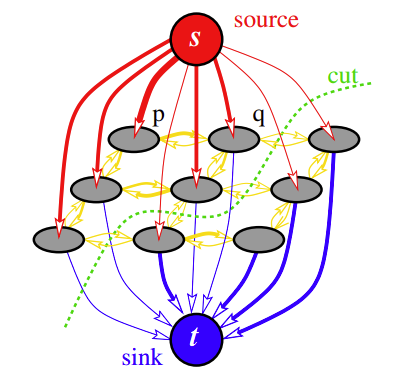
\includegraphics[width=0.3\textwidth]{images/graph_cut}
    \caption{Приклад графу-решітки з мінімальним розрізом
    \label{fig:graph_lattice}
    }
\end{figure}

Найбільша перевага даного алгоритму це те що, він працює швидше та краще на графах-решітках 
(рис.\ref{fig:graph_lattice}).
Оскільки саме таку структуру ми використовуємо в алгоритмі Б-К для отримання маски рухомих 
об'єктів це дає змогу оброблювати кадри відео досить шивдко.
